\section{Taxonomy based joins for single match}
\label{sec:taxo_similarity}

In this section, we investigate a special case when a string matches only one node in a taxonomy tree, which will form a foundation to a generalised case studied in the next section.

\subsection{Similarity functions}

Given a taxonomy tree, we borrow an existing labelling scheme called \textit{Dewey code}, which is a prefix-based scheme that records the position of each node, according to the path from the root to the node. The IS-A relations between tree nodes can be determined easily. For example, Figure \ref{fig:toytaxonomyexample} shows an example of a taxonomy tree with Dewey codes. ``\textsf{California} (2.1.1.1)'' IS-A part of ``\textsf{U.S.} (2.1)'', because ``2.1'' is the prefix of ``2.1.1.1''. Based on the Dewey code, we can define the similaity between two nodes in a taxonomy tree as follows.



Given two nodes $n_1$ and $n_2$ labeled with Dewey codes on a taxonomy tree, the taxonomy similarity (TS) between $n_1$ and $n_2$,

\begin{equation}
 TS_{max}(n_1,n_2) = \frac{|LCP(n_1,n_2)|}{max(|n_1|,|n_2|)}
\end{equation}

\smallskip
\smallskip


One of the most popular edge counting measure is that proposed by Wu and Palmer \cite{conf/acl/WuP94} as follows:

\begin{equation}
TS_{sum}(n_1,n_2) = \frac{2|LCP(n_1,n_2)|}{|n_1|+|n_2|}
\end{equation}

The measure based on information content have a similar structure but instead of using the depth in the taxonomy they use an estimation of the information carried by the concpet. Different measures are characterized by different ways of estimating the information content, using either a data corpus or the intrinsic structure of the taxonomy.  A method which uses only the taxonomy structure has been proposed in \cite{journals/kbs/SanchezBI11}  where the information content of a concpet is expressed as the ratio between a measure of its generality (relatd to the number of ancestors) and a measure of its concreteness (related to the number of descendants). The specfic estimation of the information conetnt is described in Eq.



\begin{equation}
TS_{IC}(n_1,n_2) = \frac{2IC(LCP(n_1,n_2))}{IC(n_1)|+IC(n_2)}
\end{equation}


\begin{equation}
IC(n) = -log (\frac{|Leaves(n)|/|Ancestors(n)|+1}{|All~leaves|+1})
\end{equation}

\begin{example}
Consider Figure \ref{fig:toytaxonomyexample}, the similarity between ``\textsf{Seoul}'' (3.1.1.1) and ``\textsf{Suwon}'' (3.1.1.2) is $\frac{3}{4}$= 0.75 (as both countries locate in the same country: South Korea.), but the similarity between ``\textsf{Seoul}''  (3.1.1.1) and ``\textsf{Shenzhen}'' (3.2.1.1) is only $\frac{1}{4}$= 0.25 (as two countries locate in the different countries, but the same continent: Asia).
\end{example}


% In the worst case, the time complexity to compute the taxonomy similarity is linear to the length of the Dewey codes of nodes $n_1$ and $n_2$. 


\subsection{Join algorithms for sorted lists}

Given two collections of strings $S_1$ and $S_2$,  a \textit{similarity join} finds all pairs $(n_1, n_2) \in S_1 \times S_2$,
such that $TS(n_1,n_2)$ $>$ $\theta$, where $\theta$ is a predefined threshold. A baseline algorithm is the nested-loop join, which generates all string pairs to verify their similarities.  Obviously, this baseline involves many unnecessary verifications for string pairs which cannot contribute to final answers. We next propose two families of algorithms to speed up the processing.

\begin{algorithm}
{\bf Input}: two sorted lists  $L_1$ and $L_2$\\
{\bf Output}: pairs $R$ =\{$(s_1,s_2) \in L_1 \times L_2$ | $TS(s_1, s_2) > \theta$\}
\begin{compactenum}[(1)]
\item {\bf FOR}  i =1 and 2 {\bf DO}
\item ~~ Initialize two pointers $C_i^1$ and $C_i^2$ to the first element of  $L_i$
\item {\bf WHILE}  ($\neg$end($L_1$) and $\neg$end($L_2$)) {\bf DO}
\item ~~ $min$ = $\arg\min_{i}$($cur(C_i^1)$); $max$ = $\arg\max_{i}$($cur(C_i^1)$)
\item ~~ Let $p$ denotes the prefix of $cur(C_{min}^1)$ with the length $  \lceil l \cdot \theta \rceil$
\item ~~ $C_{max}^2$ =$C_{max}^1$
\item ~~ {\bf WHILE} ($p$ is a prefix of (cur($C_{max}^2$) ) {\bf DO}
\item ~~ ~~ ~~ {\bf IF} TS(cur($C_{max}^2$), cur($C_{min}^1$))$> \theta$ {\bf THEN}
\item ~~~   ~~ ~~ ~~ Add (cur($C_{max}^2$), cur($C_{min}^1$)) to $R$
\item ~~ ~~ ~~ advance($C_{max}^2$)
\item ~~   advance($C_{min}^1$)
\item  {\bf Return} $R$
\end{compactenum}
\caption{TS Join based on sorted labels}
\label{alg:exactjoin}
\end{algorithm}





The first optimization is to sort the lists in advance. Given a collection of strings $S$,  a list $L_S$ contains the \textit{Dewey} codes of the taxonomy tree nodes that match strings. The labels in the list are sorted by the ascending lexicographical order. The operations over lists are: \textit{advance} and \textit{end}, which move the cursor of a list to the next position and test if the cursor points to the end of a list, respectively.



Algorithm \ref{alg:exactjoin} shows the pseudo-code of a string join based on sorted lists. There are two cursors $C_1$ and $C_2$ in each list. This algorithm repeatedly finds the pairs that share the certain number of common prefixes, by iterating though the list in sorted order, and return the answers. In particular,  for each accessed node $n$ pointed by the cursor $C^1_{min}$, the algorithm read all nodes  which share the certain number of the common prefix with $n$, i.e. $ \lceil |n| \dot \theta \rceil$, which are pointed by the cursor $C^2_{max}$ and calculate the similarity between two string to find all results. In Line 5, $l$ is the length of  $cur(C^1_{min})$.

\begin{example} See Figure \ref{fig:sortJoin}(a). We use this example to illustrate Algorithm \ref{alg:exactjoin}. The join threshold is 0.6. First the two points $C_1$ and $C_2$ point to the first elements. Note that there is no LCP computation from 1.1 to 1.4. Then pointers go forward to find the pair $(1.5.4, 1.5.5.1)$. Their similarity is less than 0.6, but 2/3 $>$ 0.6. So the pointers need to visit 1.5.5.1 to 1.5.5.4. Then finally, the algorithm find the matched pairs 1.5.5 and 1.5.5.1 to 1.5.5.4.  
\end{example}

The following lemma is a key to establish the correctness of Algorithm \ref{alg:exactjoin}. The proofs and Lemma and Theorem can be found in Appendix.

\begin{lem} Given a string $s$ with the length $|s|$, if any string t, $TS(s,t) > \theta$,  then $s$ and $t$ share the prefix with the length of at least $|s| \cdot \theta $.
\label{lemma:sortjoinlength}
\end{lem}

\begin{theorem} Algorithm \ref{alg:exactjoin} correctly finds all results for the string joins. In the worst case, the time complexity is  $O(|L_1| \cdot |L_2| \cdot n)$, where $n$ is the length of the longest string. \label{theo:sortedjoin}, $|L_1|$ and $|L_2|$ denote the cardinality of two lists.
\end{theorem}




\begin{algorithm}
{\bf Input}: two sorted lists  $L_1$ and $L_2$\\
{\bf Output}: pairs $R$ =\{$(s_1,s_2) \in L_1 \times L_2$ | $TS(s_1, s_2) > \theta$\}
\begin{compactenum}[(1)]
\item {\bf FOR}  i =1 and 2 {\bf DO}
\item ~~ Initialize two pointers $C_i^1$ and $C_i^2$ to the first element of  $L_i$
\item Let $x$ = $|LCP(cur(C_1^1),cur(C_2^1))|$
\item $min$ = $\arg\min_{i}$($cur(C_i^1)$); $max$ = $\arg\max_{i}$($cur(C_i^1)$)
\item {\bf WHILE}  ($\neg$end($L_1$) and $\neg$end($L_2$)) {\bf DO}
\item ~~ $C_{max}^2$ =$C_{max}^1$
\item ~~ $y = x$
\item ~~ {\bf WHILE} ($y \geq \lceil |cur(C_{min}^1)| \cdot \theta  \rceil$) {\bf DO}
\item ~~ ~~ ~~ {\bf IF} ($\frac{y}{max(|cur(C_{max}^2)|,|cur(C_{min}^1)|)}$ $> \theta$) {\bf THEN}
\item ~~ ~~ ~~ ~~ ~~ ~~ Add  the pair ($cur(C_{max}^2),cur(C_{min}^1)$) to $R$
\item ~~ ~~ ~~  advance($C_{max}^2$)
\item ~~ ~~ ~~ {\bf IF} $y > LP(C_{max}^2)$  {\bf THEN} $y$ = $LP(C_{max}^2)$
\item ~~ advance($C_{min}^1$)
\item ~~  {\bf IF} $x > LP(C_{min}^1)$  {\bf THEN}
\item ~~ ~~ ~~ $x$ = $LP(C_{min}^1)$ and exchange the values of $min$ and $max$
\item ~~ ~~ {\bf ELSE IF}  $x == LP(C_{min}^1)$  {\bf THEN}
\item ~~ ~~~~ ~~~~ ~~ recompute $x$, $min$ and $max$ as Lines (3) and (4)
\item {\bf Return} R
\end{compactenum}
\caption{Optimized TS Join based on sorted labels}
\label{alg:LCPSortJoin}
\end{algorithm}


 Algorithm \ref{alg:exactjoin} needs to compare two strings frequently  in Lines 4,7 and 8. When the string is long, this may takes a lot of time. We next propose an optimization to speed up this processing.

 We employ an index called  $LP(n)$, which is the length of the LCP between the node n and its preceding node. See the node ``1.1.2'' in the list $L_1$ of Figure \ref{fig:sortJoin}. LP(1.1.1) = 2, since LCP(1.1.1,1.1.2)=2.  We now introduce an algorithm to reduce the number of string comparison in Algorithm 2. Similar to Algorithm \ref{alg:exactjoin}, we maintain two cursors C1 and C2 for each list. But the main difference between Algorithm 2 and Algorithm 1 is that we avoid the prefix checking to compute the LCP. Unlike Line 7 in Algorithm 1, Algorithm 2 do not compute LCP and compare the length of strings. We use the preprocessing LCP values and avoid the computation of LCP in most cases. Therefore, we achieve better performance.
 
 We now go through Algorithm \ref{alg:LCPSortJoin}. In Line 1 and 2, it initialize two pointers for each list. In line 3, x denotes the length of LCP of two current elements. Line 4 compute the current min and max element. In Line 5 to 17, it iteratively access all elements in two lists. Line 6, set two pointers in the max list to be equal. y is a variable to recode the the length of LCP for two elements in the  $cur(C_{max}^2$) and $cur(C_{min}^1)$. In Line 9 and 10, we do not need to compute LCP, but we can know the results. The correctness can be proved in Lemma. In Line 12, update the length of LCP, but we can directly derive from LP. In line 14 to 17, update the length of LCP for two current element pointed by  $cur(C_{i}^1)$. The correctness can be proved in Lemma .
 
 z is the necessary prefix to satisfy the similarity. In Line 8, if the length of the two elements satisfy the condition in Line 9, we do not need to compute the similarity, but directly add them to the result R. Line 11 consider the next element and update the LP (reduce it if necessary). Line 12 to 19 recompute the LCP to x. If $x <> LP(C_{min}^1)$, we can avoid the LCP computation. We can save the cost a lot in this step.  

%\begin{figure}[t]
%	\centering
%	\includegraphics[width=0.22\textwidth]{figures/joinExample}
%	\caption{Illustration to join algorithm}
%	\label{fig:join}
%\end{figure}
%
%\begin{figure}
%	\centering
%	\includegraphics[width=0.5\textwidth]{figures/figureExampleRef}
%	\caption{Illustration to join algorithm}
%	\label{fig:triejoin}
%\end{figure}
%
%\begin{figure}
%	\centering
%	\includegraphics[width=0.25\textwidth]{figures/trieExample}
%	\caption{Illustration to join algorithm}
%	\label{fig:triejoin}
%\end{figure}


\begin{figure}[t]
\centering
\includegraphics[width=0.5\textwidth]{figures/joinExample2}
 \caption{Illustration to the optimized sorted join algorithm. Each item is a binary tuple: (Dewey, LP). The join threshold $\theta >$ 0.6 }
\label{fig:sortJoin}
\end{figure}

\begin{example} We use this example to illustrate Algorithm \ref{alg:LCPSortJoin}. Compared to Algorithm 1. the main difference is that we can avoid the computation of LCP from 1.5.5.2 to 1.5.5.4, since we LP=3, we can advance it in Line 14. When the list is long, it can save more computation of LCP. 
\end{example}

The following lemma is a key to establish the correctness of Algorithm \ref{alg:LCPSortJoin}.

\begin{lem} Let A, B and C be three Dewey codes,

(a) If $LCP(A,B) \neq LCP(B,C)$,  then $LCP(A,C)$ = min\{$LCP(A,B)$, $LCP(B,C)$\}.

(b) If $A>B$, $C>B$ and $|LCP(A,B)|>|LCP(B,C)|$ , then $C>B$.
\label{lemma:LCPcomparison}
\end{lem}

\begin{theorem} Algorithm \ref{alg:LCPSortJoin} correctly finds all results for the string joins. \label{theorem:LCPSortCorrectness}
\end{theorem}


We can show that the worst time complexity is bounded by the product of the size of two collections plus with a sum of LCP array, which is defined as the LCP sum of alternative elements, which is better than Algorithm 1.



\begin{definition} [LCP Array] Given two sorted sets of Dewey codes $S_1$ and $S_2$, first merge and sort $S_1$ and $S_2$ to one list S=$S_1 \cup S_2$, and for an elment $i$ in S, is the length of the LCP with the previous one for the element i in S, denoted as $LCPA_i(S1,S2)$.
\end{definition}

\smallskip

\begin{theorem} The TS join based on LP perform the join for two tables $T_1$ and $T_2$ in the worst complexity is $\mathcal{O}$$(S+|T_1||T_2|)$, where S= $\Sigma LCP(e,e')$, $e$ and $e'$ are two adjacent labels from the different tables in the merged sorted list.
\end{theorem}

\smallskip

Algorithm \ref{alg:LCPSortJoin} improves Algorithm \ref{alg:exactjoin} by reducing the cost for prefix computations. Unfortunately, Algorithm \ref{alg:LCPSortJoin} is not guaranteed to be optimal, in that the computation cost is not bounded by the size of input and output data. See an example of sub-optimality as follow. Recall Figure \ref{fig:sortJoin}. There are no answers for 1.5.4, and the accesses from 1.5.5.1 to 1.5.5.4 are useless. Therefore, this is not an optimal algorithm. In the next section, we seek to overcome this sub-optimality using a compact trie.

\subsection{Join algorithms with compact tries}

 Trie is a rooted tree with the following properties: Edges are labelled with symbols from an alphabet $\Sigma$. For every node $v$, the edges from $v$ to its children have different labels. Each node represents the string obtained by concatenating the symbols on the path from the root to that node. Compact tries reduce the number of nodes by replacing branchless path segments with a single edge. There are two kinds of nodes in compact trie. One is the real number with rectangle. The other is the internal node, which add an integer to indicate the shortest real element under the subtree. The construction and maintenance of a TC-trie is very similar to those in a compact trie, using the prefix as the key; the difference is that the I values in the internal node need to be propagated up the index structure.

%\begin{figure}[t]
%\centering
%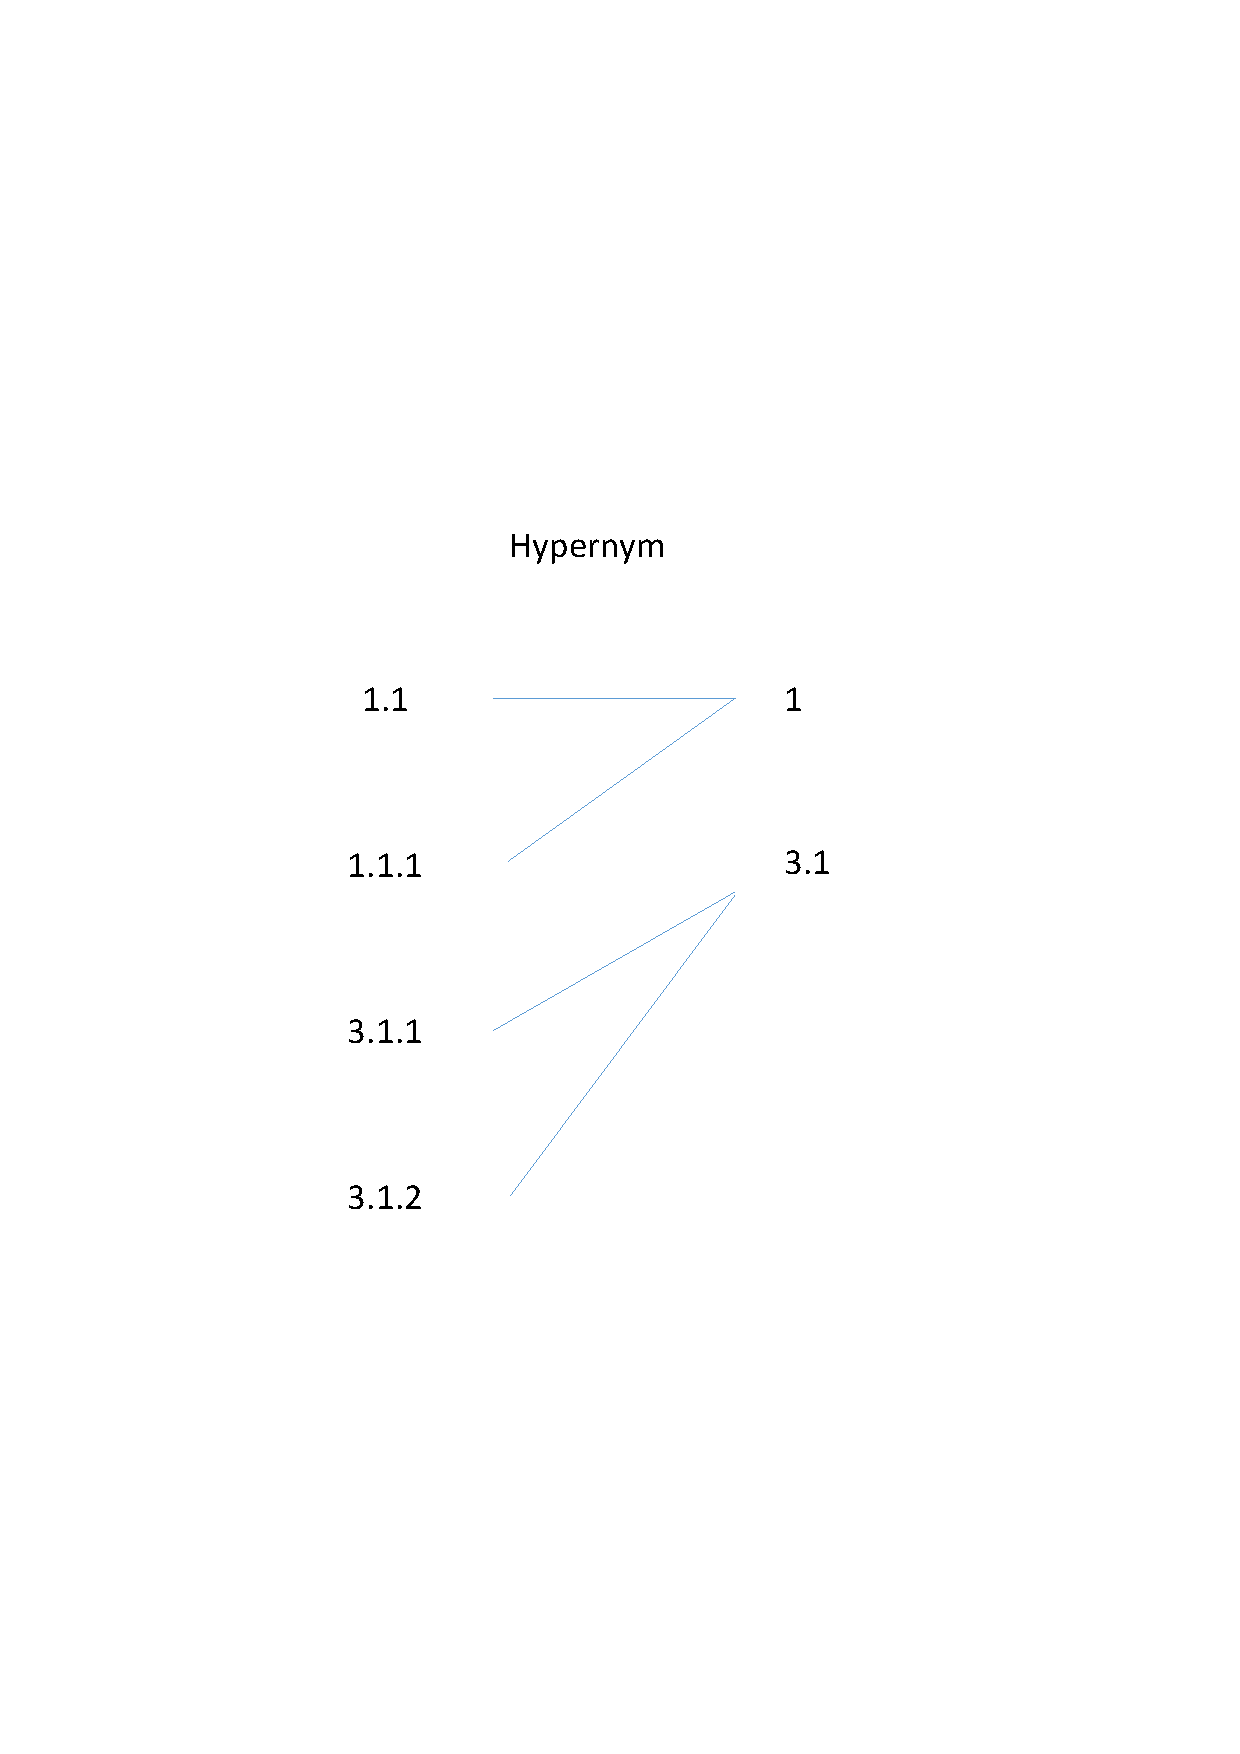
\includegraphics[scale=0.4]{figures/labeljoins}
% \caption{Join inverted lists}
%\label{fig:invertedlist}
%\end{figure}

%The worst case complexity is $O(N^2)$, because the algorithm may compute each pair of strings with the prefix $p$. But this algorithm will skip many pairs of string for comparison. A theoretical analysis based on a random string model show that the average complexity is $O(\frac{N^2}{S^{\lfloor (1-\theta) \cdot l \rfloor}})$, where $N$ is the total number of elements in each list and $S$ is the maximal width of the taxonomy.




%\begin{figure}[t]
%\centering
%\includegraphics[width=0.35\textwidth]{figures/prefixTrees}
% \caption{An example of TS join based on prefix trees (a circle means an internal element, but a rectangle means a real element)}
%\label{fig:taxonomyexample}
%\end{figure}



\begin{algorithm}
{\bf Input}: two collections of taxonomy nodes $S_1$ and $S_2$,  a threshold $\theta$ \\
{\bf Output}: string pairs $(s_1,s_2) \in S_1 \times S_2$, s.t. $TS(s_1, s_2) > \theta$
\begin{compactenum}[(1)]
\item Let $T_s$ and $T_t$ denote two compact tries for $S$ and $T$ respectively.
\item Initialize two cursors in two tries to point to the first real nodes
\item {\bf WHILE} ($\neg end(T_s) \wedge  \neg end(T_t)$) {\bf DO}
\item  ~~ $min$ = $\arg\min_{i}$($cur(C_i)$); $max$ = $\arg\max_{i}$($cur(C_i)$)
\item  ~~ {\bf IF} (possibleMatch(cur($T_{min}$),cur($T_{max}$))) {\bf THEN}
\item ~~ ~~ {\bf  IF} ($cur(T_{min})$ is an element)  {\bf THEN}
\item ~~ ~~  ~~ ~~ getResults(cur($T_{min})$,cur($T_{max}$))
\item ~~~~ advance($T_{min}$)
\item ~~ {\bf ELSE} Jump($T_{min}$)
\end{compactenum}
\smallskip
\textbf{Function} possibleMatch($s_1$,$s_2$)
\begin{compactenum}[(1)]
\item  $x =| LCP(s_1,s_2) |$
\item {\bf IF}  $x > \theta \cdot max (s_1, s_2 )$  {\bf THEN} RETURN TRUE
\item   ~~ {\bf ELSE} RETURN FALSE
\end{compactenum}
\smallskip
\textbf{Procedure} Jump($T$)
\begin{compactenum}[(1)]
%\item  read the next real node that is not a descendant of $cur(T)$ with the depth-first traversal
\item  find the smallest real node in T which share at least  $\theta cur( T_{max}$) 
\end{compactenum}
\smallskip
\textbf{Procedure} getResults($s_1$,$s_2$)
\begin{compactenum}[(1)]
\item  {\bf FOR EACH} ancestor $p$ (including $s_2$) of $s_2$ in  $T_{max}$ {\bf DO}
\item   ~~~ $x=LCP(p,s_1)$
\item   ~~~ {\bf FOR EACH} real nodes $s_i$ of the descendants of $p$  s.t.  $s_i > s_2$ and $|s_i| <= \lfloor |x|/ \theta \rfloor $ {\bf DO}
\item ~~~~~~~~ Add ($s_1,s_i$) to $R$;
\end{compactenum}
\caption{String joins with compact tries}
\label{alg:compactTrieJoin}
\end{algorithm}


We maintain a pointer $C$ to the node in TC trie. There are two operations over the TC-trie that affects this pointer:

1. \textsf{Advance} We advance $C$ to the next node in the trie with depth-first traversal.

2. \textsf{Jump} We jump $C$ to the right sibling node.

Initially $C$ points to the root node of TC trie. When C points to the last node in two TC tries and we advance it, we finish the traversal.

Algorithm \ref{alg:compactTrieJoin} shows the pseudo-code for string join with compact tries. The main idea is to use the trie to skip the nodes which cannot contribute to the final results. We  go through the algorithm. Line 5 determine if the current two elements can match. If yes, then we get results and then adance the minimal element. In line 7, we access the tree to find all element which can match $cur(C_{min})$. In Procedure getResults, we access the descendant of p only if there exists a node by minLen which is less than $ \lfloor |x|/ \theta \rfloor $.


\smallskip
\smallskip

\begin{example}
Consider the example in Figure \ref{fig:sortJoin}c, $\theta$=0.6. First, the cursors point to 2 and 2. possibleMatch return true. Compared to previous example, note that the accesses from 1.5.5.1 to 1.5.5.4 fro 1.5.4 are jumped. Therefore, it is optimal for this case.
\end{example}

\smallskip
\smallskip


\begin{theorem} Given two collections of nodes and a threshold $\theta$, Algorithm \ref{alg:compactTrieJoin} correctly finds all pair $n_1$ and $n_2$ such that $TS(n_1,n_2) > \theta$.
\end{theorem}

The correctness of the above theorem and the procedure of \textit{getResults} in the algorithm is based on the following lemma:

\begin{lem} Given two labels $s$ and $t$,  assume that $LCP(s,t) = x$. without the loss of generality, assume that $s<t$ by the lexicographical order, $TS(s,t) > \theta$ if and only if  $ x > \theta |s| $ and $  |t| < max(\frac{x}{\theta},|s|)$.
\end{lem}
\begin{proof}  $TS(s,t) > \theta$ $\Leftrightarrow$ $\frac{x}{|s|+|t|-x} > \theta \Leftrightarrow |t| < (\frac{1}{\theta}+1)x-|s|$. In addition, note that $|t| \geq x$. Then $x < (\frac{1}{\theta}+1)x-|s|$ $\Rightarrow$ $x > \theta |s| $, which concludes the proof.
\end{proof}


We next show the optimality: Given two compact tries, Algorithm \ref{alg:compactTrieJoin} takes each node and find the  matching node with the trie operations. Therefore, each accessed pair $C_1$ and $C_2$ belong to the final results. Since the operation of output Line is equal to the size of the final results: we have the following optimality result:

\begin{theorem}   The computing cost of Algorithm \ref{alg:compactTrieJoin} is linear to the sum of the size of the input and output. \label{theo:optimality_compactTrie}
\end{theorem}

\begin{proof}  The algorithm finds an answer in Procedure finds. Therefore, the optimality can be guaranteed.
\end{proof}


